\newpage 
\section{Stochastic differential equation}
\begin{rem}
Considering all differential equations, one first has to define a solution (What does it means to be a solution of DE), generally, we need some space. And next step will be finding the conditions about existence and uniqueness, perhaps continuous or Lipschitz continuous. Understand that there are no "minimal" conditions since there is no way to define "minimality". It always starts with the question "What types of solutions we are looking for" and then we try to define the conditions for solutions.

The second remark is about the conditions, all the conditions we assumed here are in some sense "Strong", but again, there is no "minimality", remember, some conditions here can actually be dropped (like linear growth rate conditions). 
\end{rem}

\subsection{Preparation work}
Before we consider the theory of SDE, we first give some well-known facts:

\begin{thm}{(Levy characterisation theorem)}

Let $(M_t, \F_t)$ be continuous local martingale with $\qvar{M}{t} = t$ then $(M_t, \F_t)$ is Brownian motion.
\end{thm}

\begin{example}
$M_t = \int_0^t sgn(W_s) \diff W_s$.
\end{example}
\begin{lem}
For multidimensional case, $(M_t, \F_t)\in \R^d$ continuous local martingale with $\qvar{N^i, M^j}{t} = t\delta_{i,j}$ then $(M_t, \F_t)$ is Brownian motion.
\end{lem}

\begin{thm}{(Time change)}\label{Thm: time_change}

Let $M_t = \int_0^t F_s \diff W_s, \int_0^t \abs{F_s}^2 \diff s < \infty, \forall t$ then $(M_t, \F_t) $ is continuous local martingale and $\qvar{M}{t} = \int_0^t \abs{F_s}^2 \diff s$, then there exists a BM $(B_t)$ s.t
\begin{equation*}
    M_t = B_{\qvar{M}{t}}.
\end{equation*}
\end{thm}

We have a few remarks: This gives a new-looking perspective of local martingales, they are always some time changes of some Brownian motion but the relationship between $B_t, W_t$ is not clear.

\begin{example}
See Assignment 1 Q2, another application see Tut9 Q4.
\end{example}

\begin{thm}{(Martingale-representation theorem)}

Let $(\Omega, \F_t^W, \prob)$ be probability space but notice the filtration is generated by BM. Let $X\in \ls{2}, X\in \F_T^W$ then we have a \textit{unique} process $(h_t, \F_t^W), h \in \lp{2}$ s.t.

\begin{equation*}
    X = \E(X)+\int_0^T h_s \diff W_s.
\end{equation*}
\end{thm}

\begin{lem}
Let $(M_t, \F_t^W)$ be a square-integrable martingale, $t\in[0,T]$ then there exists a unique $\F$ predictable process $(h_s) \in \lp{2}, s\leq T$, such that 

\begin{equation*}
    M_t = M_0 + \int_0^t h_s \diff W_s.
\end{equation*}
\end{lem}

See Marek's notes on page 21 for details.

\subsection{Standard SDE}

$(\Omega, \F, (\F_t), \prob)$ be given, $(W_t, \F_t)$ be $R^d$ valued BM. SDE is an equation with the following form
\begin{equation*}
    X_t = \eta + \int_s^t F(r,X_r) \diff r+\int_s^t G(r,X_r) \diff W_r,
\end{equation*}
where $F(t,X_t)$ is local drift and $G(r,X_r)$ is local diffusion. Intuitively, local drift is the local "velocity" of the process, local diffusion is local variance. In differential form,
\begin{equation*}
    \begin{cases}
        \diff X_t = F(t,X_t) \diff t + G(t,X_t) \diff W_t \\
        X_s = \eta,\quad  s\leq t \leq T.
    \end{cases}
\end{equation*}

\begin{dfn}{(Space $C_b$)}

We define the space $C_b([0,T], \ls{2}(\Omega,\F,\prob))$, a process $(X_t)\in C_b$ if it is progressively measurable adapted process with norm

\begin{equation*}
    \norm{X_t}^2 = \sup_{t\leq T}\E\abs{X_t}^2 <\infty.
\end{equation*}

\end{dfn}

\begin{rem}
This space $C_b$ in Banach space.
\end{rem}

\subsubsection{Existence and uniqueness}
If it is a solution if every term should well define $F,G$ process and $\eta$ and the dynamics are satisfied for a more detailed version see Week 5 lec 1.

\begin{assmp}\label{condition1}

We require a few technical assumptions in order to guarantee existence and uniqueness.
\begin{itemize}
    \item $F,G$ are continuous on $[0,T]\times \R^d$.
    \item Lipschitz continuous condition: $\exists M_L$ s.t.
    \begin{equation*}
        \abs{F(t,x)-F(t,y)}^2 + \norm{G(t,x)-G(x,y)}^2 \leq M_L^2 \abs{x-y}^2
    \end{equation*} $\forall t\in[0,T], \forall x,y\in \R^d$.
    \item Linear growth rate (Not necessary)
    \begin{equation*}
        \abs{F(t,x)}^2 + \norm{G(t,x)}^2 \leq M_L^2(1+\abs{X}^2) \quad t\in[0,T], \forall x\in \R.
    \end{equation*}
\end{itemize}
\end{assmp}

\begin{thm}
Assume that $\eta\in\F_s$ and square-integrable and assumption \ref{condition1} satisfied. Then there exists a unique solution to (SDE) denoted as $X(t,s,\eta), t\in[s,T]$.
\end{thm}
The proof is based on the Banach Fixed point theorem, omitted here.

\begin{thm}{(Banach Fixed point)}

Let $E$ be a Banach space and define $K: E\rightarrow E$ be contraction:
\begin{equation*}
    \norm{K(x)-K(y)} \leq \alpha \norm{x-y}\quad \forall x,y\in E, \alpha \in (0,1).
\end{equation*}

Then there exists a \textit{unique} point $x_0\in E$ s.t.
\begin{equation*}
    K(x_0) = x_0.
\end{equation*}
\end{thm}

Next, we formulate the proof in following steps and leave the details. \\
\textbf{Idea: }

Define $KX_t = X_t = \eta + \int_s^t F(r,X_r) \diff r+\int_s^t G(r,X_r) \diff W_r$.

\textbf{Step1: }

We know the process in $C_b$ is a Banach space.
Show $K: C_b \rightarrow C_b$.

\textbf{Step2: }

Show the operation $K$ we define is a contraction, that is:
\begin{equation*}
    \norm{K(x)-K(y)} \leq \alpha \norm{x-y}\quad \forall x,y\in C_b, \alpha \in (0,1).
\end{equation*}

\textbf{Step3: }

Now using the Banach Fixed point theorem, we conclude there exists a unique point(process) in $C_b$ s.t \begin{equation*}
    KX_t = X_t = \eta + \int_s^t F(r,X_r) \diff r+\int_s^t G(r,X_r) \diff W_r
\end{equation*} as desired.
\qed

\begin{rem}
In step 2 proof, we need to choose $T$ to make sure $\alpha \in (0,1)$ which might not be the desired $T$ in the first place. The idea will formulate another equation take the initial condition of a process $X_t$ as $X_T$ of the previous one, and use a similar argument to continue this argument until terminal time. Also, this choice of $T$ does not depend on the initial condition which is also essential here, now we have linear growth in time $T+ T+ T + ...$, with no question of convergence.
\end{rem}

\subsubsection{Picard Iteration}
\begin{prop}
The start will any point in $C_b$ will end up at the unique point which is the solution. We define the sequence $(X_n)$ by setting $X_0 = 0$ and for every $n = 1,2,3,...$
\begin{equation*}
    \begin{cases}
    X_t^{n+1} = X_t^n = \eta + \int_s^t F(r,X_r^n) \diff r+\int_s^t G(r,X_r^n) \diff W_r \\
    X_t^{n+1} = \eta
    \end{cases}
\end{equation*}
Then the sequence converges in $C_b$ a.e.
\end{prop}

\subsubsection{Properties}
\begin{lem}{(Co-cycle rule)}\\
Let's denote $X(t,s,\eta)$ as the solution at time $t$ starting from $s$ with initial condition $\eta$, then by uniqueness of solution we have
\begin{equation*}
    X(t,s,\eta) = X(t,r, X(r,s,\eta)), 0 \leq s \leq r \leq t \leq T.
\end{equation*}
\end{lem}

\subsubsection{Prior estimates}\label{Sec: prior_estimate}
Consider the "function" $(t,s, \eta) \xrightarrow{X} X(t,s,\eta)$. Now we want to study what will change or in what rate of change if we change the time scale. Will the solution be stable? 
\begin{lem}{(Prior estimates of $X$)}
\begin{equation*}
    \E\abs{X(t,s,\eta)}^2 \leq 3e^{3M_L^2(T-s+1)}\left( \E\abs{\eta}^2 + M_L^2(T-s)^2 + T-s \right).
\end{equation*}
If you change the initial condition, the solution will be bounded in the square in sense.
\end{lem}

\begin{lem}{(Change terminal time)}

Let $0\leq s \leq t_1 < t \leq T$ then
\begin{align*}
    \E\norm{X(t,s,\eta) - X(t_1, s, \eta)}^2 &\leq  2M_L^2(t-t_1)^2+(t-t_1)(1+C_{T,\eta}^2) \\
    &\leq A_{T,\eta}(t-t_1).
\end{align*}
\end{lem}


\begin{lem}{(Change initial condition)}

Let $\eta, \xi \in \ls{2}$ and $\F_s$ measurable then
\begin{equation*}
    \E\norm{X(t,s,\eta) - X(t, s, \xi)}^2 \leq  3e^{3M_L^2(T-s+1)(t-s)} \E\abs{\eta-\xi}^2.
\end{equation*}
\end{lem}

\begin{lem}{(Change initial time)}

Let $0\leq s \leq s_1 < t \leq T$ then
\begin{align*}
    \E\norm{X(t,s,\eta) - X(t, s_1, \eta)}^2 \leq \hat{C}_{T,\eta}\abs{s-s_1}.
\end{align*}
\end{lem}

\pf This proof can be converted into the previous lemma by the Co-cycle lemma in the following way
\begin{equation*}
    X(t,s,\eta)-X(t,s_1,\eta) = X(t,s_1,X(s_1,s,\eta))-X(t,s_1,\eta),
\end{equation*}
then the only difference is at the initial condition.
\begin{align*}
    \E\norm{X(t,s,\eta) - X(t, s_1, \eta)}^2 &= \E\norm{X(t,s_1,X(s_1,s,\eta))-X(t,s_1,\eta)}^2 \\
    & \leq C_T \E\abs{X(s_1,s,\eta) - \eta} = C_T \E\abs{X(s_1,s,\eta) - X(s,s,\eta)}
    \intertext{Now the difference is at terminal time}
    &\leq \hat{C}_{T,\eta}\abs{s_1 -s}.
\end{align*}
\qed

\subsubsection{Regularities}
Next, we study the properties of differentiability of function $(t,s, \eta) \xrightarrow{X} X(t,s,\eta) \in \ls{2}$.

\begin{equation*}
    X_t = \eta + \int_s^t F(r,X_r) \diff r+\int_s^t G(r,X_r) \diff W_r.
\end{equation*}

Then we consider the function change in the forward and backward direction.
\begin{itemize}
    \item $x\rightarrow X(t,s,x), t,s$ fixed.
    \item $s\rightarrow X(t,s,x), t,x$ fixed (tricky requires backward \ito).
\end{itemize}

\begin{assmp}\label{condition2} 

Recall we have some assumptions on $F, G$ at \ref{condition1} to make sure of the existence of the solution, in order to obtain differentiability we need $F, G$ to be continuously bounded for first, second derivative w.r.t $x$.
\begin{itemize}
        \item For $x\in \R^d, k=1,2$ 
        \begin{align*}
            &\sup_{t\leq T}\abs{\frac{\partial^k}{\partial x_i} F(t,x)} \leq C_1.\\
            &\sup_{t\leq T}\abs{\frac{\partial^k}{\partial x_ix_j} g(t,x)} \leq C_2.
        \end{align*}
    \item Or equivalently:
    \begin{equation*}
        \sup_{t\leq T}\sup_{x\in\R^d}\abs{\frac{\partial}{\partial x_i} F(t,x)} + \sup_{t\leq T}\sup_{x\in\R^d}\abs{\frac{\partial^2}{\partial x_ix_j} g(t,x)} <\infty.
    \end{equation*}
\end{itemize}
    
\end{assmp}
Recall the function:
\begin{equation*}
    X_t = \eta + \int_s^t F(r,X_r) \diff r+\int_s^t G(r,X_r) \diff W_r.
\end{equation*}

\begin{thm}\label{Thm: directional}

Given extended fixed point theorem and little proof \footnote{See Week 5 lec 2 recording}, then the mapping $x\rightarrow X(t,s,x)$ is differentiable at every point $x\in\R^d$ in every direction $h\in\R^d$ with derivative: $\eta^h(t,x) := (\nabla X)h$ is a unique solution of
\begin{equation*}
    \begin{cases}
    \diff \eta_t^h = [\nabla F(t,X_t)]\eta_t^h \diff t + [\nabla G(t,X_t)]\eta_t^h \diff W_t \\
    \eta_s^h = h &s\leq t\leq T.
    \end{cases}
\end{equation*}
\end{thm}

Unique since the 2nd derivative is uniformly bounded, thus itself bounded, we have a unique solution since it satisfies assumption \ref{condition1}.

\textbf{Regularities of directional derivative}
\begin{lem}
We could find regulations for the fourth power of $\eta_t^h$ by using the next lemma.
\begin{equation*}
    \sup_{t\leq T} \E\abs{\eta_t^h}^4 \leq C_T \abs{h}^4.
\end{equation*}
\end{lem}We need the following lemma:
\begin{lem}
Let $\E\int_0^T \norm{F_t}^{2m} \diff t < \infty, \quad m = 1,2,,...$, then for $X_t = \int_0^t F_s \diff W_s$ we have
\begin{equation*}
\E\abs{X_t}^{2m} \leq C_m \E\int_0^T \norm{F_t}^{2m} \diff t.
\end{equation*}
\end{lem}

\pf Idea:

\textbf{Step1.} We start with case $m=2$ and do the rest by induction.

\textbf{Step2.} Assume $X_t$ is bounded s.t. $\abs{X_t} \leq C$ a.s. then we could find
\begin{equation*}
    \E\abs{X_t}^4 \leq \E\int_0^t e^{3(t-s)} \norm{ F_s}^4 \diff s \leq e^{3T} \E\int_0^T\norm{ F_s}^4 \diff s.
\end{equation*}

\textbf{Step3.} Let $X_t$ be arbitrary, and define $\tau_n = \inf\{t\geq 0; \abs{X_t}\geq n\}$, then
\begin{equation*}
    \E\abs{X_t}^4  = \E\abs{\biglim{n\rightarrow \infty} X_{t\wedge \tau_n}}^4 \leq \biglim{n\rightarrow \infty} \E\abs{ X_{t\wedge \tau_n}}^4 \leq e^{3T} \E\int_0^T\norm{ F_s}^4 \diff s
\end{equation*} by Fatou's lemma.

Now we provide the proof of the previous lemma: 
\begin{equation*}
    \eta_t^h = h + \int_0^t F_x(X_s) \eta_s^h \diff s+\int_0^t G_x(X_s) \eta_s^h \diff W_s,
\end{equation*}
\begin{align*}
    \abs{\eta_t^h}^4 &\leq 3^3\left[\abs{h}^4 + \abs{\int_0^t F_x(X_s) \eta_s^h \diff s}^4 + \abs{\int_0^t G_x(X_s) \eta_s^h \diff W_s}^4\right], \\
    \E\abs{\eta_t^h}^4  &\leq 3^3\left[\abs{h}^4 + \E \abs{\int_0^t F_x(X_s) \eta_s^h \diff s}^4 + \E \abs{\int_0^t G_x(X_s) \eta_s^h \diff W_s}^4\right].
\end{align*}
Note, the partial derivatives are bounded, 
\begin{equation*}
    \E \abs{\int_0^t F_x(X_s) \eta_s^h \diff s}^4 \leq C_1 \E \abs{\int_0^t \eta_s^h \diff s}^4 \leq C_1' \int_0^t \E\abs{\eta_s^h}^4 \diff s.
\end{equation*} The second step could be justified by Cauchy-Schwarz inequality.
\begin{equation*}
    \E \abs{\int_0^t G_x(X_s) \eta_s^h \diff W_s}^4 \leq C_2 \E\int_0^t \abs{ G_x(X_s) \eta_s^h }^4\diff s \leq C_2' \int_0^t\E \abs{\eta_s^h }^4\diff s.
\end{equation*} First inequality, by previous lemma, second inequality, partial derivatives is bounded. Finally, we get 
\begin{equation*}
    \E\abs{\eta_t^h}^4 \leq c\abs{h}^4 + c\int_0^t \E\abs{\eta_s^h}^4 \diff r
\end{equation*}
by Gronwall inequality we have the desired result.

\begin{rem}
The second order of derivative can also be well defined, but this is omitted. Because it is rather tedious and boring.
\end{rem}

\textbf{Next we go back in time To see why this is tricky, consider}   
\begin{equation*}
    \diff X_t = F(t,X_t) \diff t, \quad X_s = x,
\end{equation*} We have co-cycle property:
\begin{equation*}
    X(t,s,x) = X(t,r,X(r,s,x)),
\end{equation*}
taking derivative w.r.t $r$ gives
\begin{equation*}
    0 = X_s(t,r,X(r,s,x)) + X_x(t,r,X(r,s,x))X_t(r,s,x),
\end{equation*}
taking $r=s$ gives
\begin{equation*}
    X_s(t,s,x) =- X_x(t,s,x)F(s,x) \implies X(t,s,x) = -x -\int_s^t  \boxed{X_x(t,r,x)}F(r,x) \diff r.
\end{equation*}
\textbf{Note: }The boxed term depends on "future information" if we include the Brownian term this is problematic. Thus we need to define backward \ito calculus. We have:
\begin{equation*}
    \int_0^T W_s \diff W_s = \frac{1}{2}(W_T^2 + T),
\end{equation*}
with properties (\ito isometry and mean value):
\begin{align*}
    \E\abs{\int_0^T F_s \diff W_s}^2 = \E \int_0^T \norm{F_s}^2 \diff s, \E\int_0^T F_s \diff W_s = 0.
\end{align*}

\subsubsection{Examples}
\begin{example}{(One Dimensional)}

One simple example will be \textit{one dimensional} then it will be in the form of GBM.
\begin{equation*}
    \begin{cases}
    \diff \eta_t = [F_x(t,X_t)]\eta_t^h \diff t + [G_x(t,X_t)]\eta_t^h \diff W_t \\
    \eta_s = 1 &s\leq t\leq T.
    \end{cases}
\end{equation*}
then we have
\begin{equation*}
    \eta_t = \exp \left[\int_s^t(F_x(r,X_r) - \frac{1}{2} \int_s^t G_x^2(r,X_r)) \diff r + \int_s^t G_x(r,X_r) \diff W_r \right].
\end{equation*}
\end{example}

\begin{example}{(Geometric Brownian Motion)}\label{Ex: GBM}

Stock price model with volatility
\begin{equation*}
    \diff S_t = \mu_t S_t \diff t + \sigma_t S_t \diff W_t
\end{equation*}
then we have a unique solution (Uniqueness is given by Lipschitz condition) 
\begin{equation*}
    S_t = s_0 \exp\left[\int_0^t (\mu_s - \frac{1}{2}\sigma_s^2) \diff s + \int_0^t \sigma_s \diff W_s \right].
\end{equation*}
\end{example}

\begin{example}{(Additive Noise)}

If the $G$ function is independent of the $X$ process, the SDE is reduced to ODE.
\begin{equation*}
    \begin{cases}
    \diff \eta_t = F_x(t,X_t)\eta_t^h \diff t \\
    \eta_s = 1 &s\leq t\leq T.
    \end{cases}
\end{equation*}
Additionally, if the matrix $F_x(t,X_t)$ is commute, then:
\begin{equation*}
    \eta_t = \exp \left[\int_s^t F_x(r,X_r) \diff r\right] h.
\end{equation*}
\end{example}
\textbf{Continue of the previous example (Ornstein–Uhlenbeckz) process.}

\begin{example}{(Solution of SDE)}\label{example: OUprocess}

If the $G$ function is deterministic (independent of $X$ process), the SDE can be reduced to ODE with a finite variation. $0\leq t\leq T$, $A,B$ being matrix.

\begin{equation*}
    \begin{cases}
    \diff X_t = A X_t(t,X_t) \diff t + B \diff W_t\\
    x_0= x \in \R^d &, W_t\in \R^d.
    \end{cases}
\end{equation*}
\begin{align*}
    X_t = x + \int_0^t A X_s \diff s+ B W_t \implies \frac{\diff Y_t}{\diff t} = x + A Y_t+ B W_t,
\end{align*} 
with $Y_t = \int_0^t X_s \diff s$ generates the solution.
\begin{equation*}
    Y_t = \int_0^t e^{(t-s)A} (x+ BW_s) \diff s.
\end{equation*}
Substitute back and use \ito formula, blablabla\footnote{See week6 lec1 40min}, at the end of the day you will find
\begin{equation*}
    X_t = e^{tA}x + \int_0^t e^{(t-s)A}B \diff W_s.
\end{equation*} Then the directional derivative $\eta_t = e^{tA}$ is obvious. Moreover
\begin{equation*}
    X_t \sim N(e^{tA}x, \int_0^t e^{sA} BB^* e^{sA^*} \diff s).
\end{equation*}

If the covariance matrix has a positive determinant, $X_t$ has density. And the covariance matrix can be calculated s.t.
\begin{align*}
    Q_t =& \E(X_t - e^{tA}x)(X_t - e^{tA})^*.
\end{align*}

If $\det(Q_t) >0$ then density is well defined as
\begin{equation*}
    p_t(x,y) = \frac{1}{(2\pi)^\frac{d}{2}}\frac{1}{\sqrt{\det(Q_t)}} \exp\left[-\frac{1}{2} \qvar{Q_t^{-1}(y- e^{t A}x), y- e^{t A}x}{} \right].
\end{equation*}
\end{example}


\subsection{Link between SDE and PDE}
Historically, one first studied PDE and this probabilistic method (Stochastic analysis even Brownian motion) was developed much later. They are somehow duality exists between PDE and SDE (for example, the Feynman-Kac formula). The theory of SDE can be seen as a peculiar method of studying SDE. 

Next, we consider the connection between PDE and SDE and we start with a deterministic example of semigroup.

\subsubsection{Deterministic case (No diffusion term)}
For $s\leq t\leq T$,
\begin{equation*}
    \frac{\diff X_t}{\diff t} = F(t,X_t)\quad X_s = x.
\end{equation*}
We take partial derivative w.r.t $r$ and let $r = s$ we have
\begin{equation*}
    \boxed{X_s(t,s,x)+X_x(t,s,x)F(s,x) = 0}.
\end{equation*}
Define $\varphi \in C_b^1(\R^d)$ (Continuous and bonded first derivative) and
\begin{equation*}
    P_{s,t}\varphi(x) := \varphi(X(t,s,x)).
\end{equation*}

\begin{rem}
This is a function with three intakes maps $(s,t,x)$ to $\varphi(X(t,s,x))$ with properties
\begin{itemize}
    \item Joint continuous.
    
    \item Linear operator such that
    \begin{equation*}
        P_{s,t}(\varphi + \lambda)(x) = (\varphi + \lambda)(X(t,s,x)) = \varphi(X(t,s,x)) + \lambda(X(t,s,x)) = P_{s,t}\varphi(x)+P_{s,t}\lambda(x).
    \end{equation*}
    
    \item Semi-group property, for $0\leq s \leq r\leq t\leq T$
    \begin{equation*}
        P_{s,t}\varphi = P_{s,r}\circ P_{r,t} \varphi.
    \end{equation*}
    The proof is trivial, just play with the definition.
    
    \item Let $\varphi \in C_b^1(\R^d)$ then we have Forward/Backward Markov equation
    \begin{align*}
        \text{(Forward)}\quad \frac{\diff}{\diff t} P_{s,t}\varphi &= (P_{s,t}\circ L(t))\varphi, \\
         \text{(Backward)} \quad \frac{\diff}{\diff s} P_{s,t}\varphi &= -(L(s)\circ P_{s,t})\varphi.
    \end{align*}
\end{itemize} 
with operator $L(t)\varphi(x) = \inner{F(s,x)}{\varphi_x(x)}.$

\textbf{Then we have important PDE equivalence} with $\varphi \in C_b^1(\R^d)$,
\begin{equation*}
    \begin{cases}
        \frac{\partial }{\partial s}u(s,x) + \inner{F(s,x)}{u_x(s,x)}=0, \\
        u(T,x) = \varphi(x).
    \end{cases}
\end{equation*}
\end{rem}

\begin{thm}{Existence and Uniqueness}

The above PDE has a unique solution $u$ with continuous $u_x$ with solution
\begin{equation*}
    u(s,x) = P_{s,T}\varphi (x).
\end{equation*}
\end{thm}

The existence can be easily verified by backward Markov property. The uniqueness is again easy, we will use the PDE in the proof to show such $u$ must have the expression $P_{s,T}\varphi(x)$.

\begin{example}{Autonomous Case}

Autonomous stands for the parameter is independent of time (invariant with time variable)
\begin{equation*}
    \frac{\diff X_t}{\diff t} = F(X_t) \quad X_s = x.
\end{equation*}

Since the dynamics are independent of time, we can always shift the process with starting time $0$, that is:
\begin{equation*}
    X(t,s,x) = X(t-s, 0, x).
\end{equation*}
This could simplify our notation to $\boxed{P_t\varphi (x) = \varphi(X(t,x))}$ by:
\begin{equation*}
    P_{s,t}\varphi (x) = P_{0,t-s} \varphi(x) := P_{t-s}\varphi(x).
\end{equation*}
Thus Semi-group property, For $0\leq s\leq t\leq T$,
\begin{equation*}
    P_{t}\varphi = P_{s}\circ P_{t} \varphi.
\end{equation*}
Let $\varphi \in C_b^1(\R^d)$, then
\begin{align*}
    \frac{\diff}{\diff t} P_{t}\varphi &= (P_{t}\circ L)\varphi = (L \circ P_{t})\varphi,
\end{align*}
with $L\varphi(x) = \inner{F(x)}{\varphi_x(x)}$.
\end{example}
Then, we could form the corresponding PDE:
\begin{equation*}
    \begin{cases}
        \frac{\partial }{\partial s}u(s,x) - \inner{F(x)}{u_x(s,x)}=0. \\
        u(0,x) = \varphi(x),
    \end{cases}
\end{equation*}
with unique solution $u(t,x) = P_t\varphi(x)$. Now $F(x)$ is independent of time, we could reverse the time and define $v(t,x) = u(T-t, x)$ then we could convert the initial condition problem to a terminal value problem or vice versa.
\begin{equation*}
    \begin{cases}
        \frac{\partial }{\partial s}v(s,x) + \inner{F(x)}{v_x(s,x)}=0. \\
        v(T,x) = \varphi(x),
    \end{cases}
\end{equation*}
with unique solution $v(t,x) = P_{T-t}\varphi(x)$.

\subsubsection{Semi-group operator with general SDE case}
For $s\leq t\leq T$,
\begin{equation*}
    \diff X_t = F(t,X_t) \diff t + G(t,X_t) \diff W_t.
\end{equation*}
Define \textbf{transition operator,}
\begin{equation*}
    P_{s,t}\varphi(x) = \E(\varphi(X(t,s,x))).
\end{equation*} 
Now we assume $\varphi \in C_b(\R^d)$ be continuously bounded with continuous derivative also bounded.

\begin{rem}
In general $\varphi$ does not have to strong as this, it could be bounded Borel function to make sure expectation is well defined.
\end{rem}
To see the idea behind the name we consider $\varphi$ be indicator function
\begin{equation*}
    P_{s,t} \I{A}(x) = \prob(X(t,s,x) \in A),
\end{equation*} 
as the "transition" probability.


To see the connection with PDE, we want to show the semigroup property
\begin{equation*}
    P_{s,t} = P_{s,r} \circ P_{r,t}.
\end{equation*}

\begin{example}
Consider an explicit function
\begin{equation*}
    \diff X_t = \diff W_t,
\end{equation*}
we can show this process have semigroup property but relies on \textbf{Markov property}.
\end{example}

Thus, next we want to show the process $X$ we start with have Markov property.\\
Consider process $X$ with initial condition be simple r.v: $\eta = \bigs{ k=1}^n x_k \I{A_k}, A_k \in \F_s$ be disjoint. Recall $P_{s,t}\varphi(x)$ as a function of three variables. That is, $P_{s,t}\varphi(\eta)$ will be a random variable because $\eta$ is r.v.
\begin{rem}
Later we will be using general measure theory argument to generalize $\eta$ to square integrable random variables. We may move the limit inside everything, since $\varphi$ is continuous and bonded, $X$ is continuous in $\eta$. So we will prove following lemma for simple r.v. but everything can be generalized to square integrable case. 
\end{rem}
Now consider process $X$ with initial condition being random variables $\eta$. We define the whole process by iterations, the key idea from Banach fixed point theorem. Now the object $\varphi(X(t,s,\eta))$ is well-defined.
\begin{lem}
For $0 \leq s \leq t \leq T$, $\eta = \bigs{ k=1}^n x_k \I{A_k}, A_k \in \F_s$.
\begin{equation*}
    X(t,s,\eta) = X(t,s,x_k)\I{A_k}.
\end{equation*}
\end{lem}
\pf This can be proved by mathematical induction relying on the iteration method. Next, we almost have Markov property.

\begin{lem}{(Baby Markov property)}
$\forall \varphi \in C_b(\R^d)$, $\varphi\in\ls{2}$ be adapted and for $0 \leq s \leq t \leq T$,
\begin{equation*}
    \E[\varphi(X(t,s,\eta)|\F_s)] = \bigs{k}P_{s,t}\varphi(x_k) \I{A_k} =  P_{s,t}\varphi(\eta).
\end{equation*}
Taking expectations from both sides give
\begin{equation*}
    \E[\varphi(X(t,s,\eta))]  =  \E[P_{s,t}\varphi(\eta)].
\end{equation*}
\end{lem}
\textbf{Remark:}  Note the nature of $P_{s,t}\varphi(X(t,s,\eta))$, it is a \yd{Random variable} defined as
\begin{equation*}
    P_{s,t}\varphi(X(t,s,\eta)) := P_{s,t}\varphi(X(t,s,x_k)) \I{A_k},
\end{equation*} but not expand process $X$ and include $\eta$ as initial condition. As we said before, we could use general measure theory to generalise to square integrable cases.
\vspace{2cm}
\begin{lem}{(Semi-group property)}
For $0 \leq s\leq r \leq t \leq T$ we have,
\begin{equation*}
    \boxed{P_{s,t} = P_{s,r}\circ P_{r,t}.}
\end{equation*}
\end{lem}
\pf 
\begin{align*}
    \boxed{P_{s,r}\circ P_{r,t}} \varphi (x) &= \E[P_{r,t}\varphi (X(r,s,x))] \\
    &= \E[\varphi(X(t,r,X(r,s,x)))] \xrightarrow{co-cycle} E[\varphi X(t,s,x)] = \boxed{P_{s,t}}\varphi(x).
\end{align*}

(Co-cycle property is given by the uniqueness of the solution.)
\qed

\begin{thm}{(Markov Property)}

For $0\leq s\leq r\leq t\leq T$, let $\eta\in \ls{2}$ and $\eta\in\F_s$ we have
\begin{equation*}
    \E[\varphi(X(t,s,\eta))|\F_r] = \E[\varphi(X(t,r,X(r,s,\eta)))] = P_{r,t}\varphi(X(r,s,\eta)).
\end{equation*}

Apply expectation we also have the semi-group property for square random variables $\eta$.
\end{thm}

Kolmogorov operator or a generator of the process
\begin{equation*}
    L(s)\varphi(x) = \frac{1}{2} Tr[\varphi_{xx}(x) G(s,x) G^*(s,x)] + \qvar{F(s,x), \varphi_x(x)}{}.
\end{equation*}

Now we define the Forward and Backward Kolmogorov/ Markov equation.

\begin{thm}
If $\varphi\in C_b^2(\R^d)$ is twice differentiable also being continuous. then $t\to P_{s,t}\varphi(x)$ and $s\to P_{s,t}\varphi(x)$ are continuously differentiable for all $(s,x)$ and

\begin{align*}
    &\frac{\diff}{\diff t} P_{s,t} \varphi = P_{s,t}L(t)\varphi, \\
    &\frac{\diff}{\diff s} P_{s,t} \varphi = -L(s)P_{s,t}\varphi.
\end{align*}
\end{thm}

\pf The proof is given by normal \ito and Backward \ito formula.

Consider following PDE
\begin{align*}
    \begin{cases}
    \frac{\partial }{\partial s} u(s,x) + [L(s) u(s, \cdot)](x) = 0, \\
    u(T,x) = \varphi(x).
    \end{cases}
\end{align*}

Let's first define what is a \textbf{solution}:

\begin{dfn}
$u$ is a solution to (PDE) if $u:[s,T]\times \R^d \rightarrow \R$ is continuous and bounded, and so are $u_x, u_{xx}$.
\end{dfn}

After this, we given essential part of the theory

\begin{thm}{(Existence and Uniqueness)}

If $\varphi\in C_b^2(\R^d)$ then the solution is given by
\begin{equation*}
    u(s,x) = P_{s,T}\varphi(x) = \E\varphi(X(T,s,x)).
\end{equation*}
\end{thm}

\pf
(Existence) 

this is trivial by backward Markov property.

(Uniqueness) 

This is interesting. Let $u$ be any solution that satisfies the PDE. Fix $0\leq r \leq s \leq T$ define $M_s = u(s,X(s,r,x))$ be a random process.
\begin{align*}
    \diff M_s =& \boxed{\frac{\partial }{\partial s}  u(s,X(s,r,x)) + L(s) u(s,X(s,r,x)) }\diff s + \qvar{u_x(s,X(s,r,x)), G(s,X(s,r,x))}{} \diff W_s \\
    =& \qvar{u_x(s,X(s,r,x)), G(s,X(s,r,x))}{} \diff W_s.
\end{align*}

The boxed part is simply zero given by PDE, moreover ($M_s, \F_s$) is a martingale and $r$ is a free variable between $0$ and $s$, taking $r=s$ and
\begin{equation*}
    M_T = u(T,X(T,s,x)) = \varphi(X(T,s,x))= \yd{P_{s,T}\varphi(x)}= u(s,X(s,s,x)) = \yd{u(s,x)}.
\end{equation*}

\subsubsection{Autonomous case}
$(F,G)$ are independent of time, but before this we have to make sure that shifts in time will not change the generic of the process. That is, if we have two process $X,Y$ defined in different probability space but governed by same dynamics, then we would hope
\begin{equation*}
    L(Y(t,s,x)) = L(X(t,s,x)).
\end{equation*} 
where $L$ stands for "Law".

\begin{thm}
Different probability space and different Brownian motions, but will same dynamics and same initial conditions, then
\begin{equation*}
    \prob(Y(t,s,x)\in A) = \prob(X(t,s,x)\in A) \quad \forall A\in \B(\R^d).
\end{equation*}
\end{thm}
\pf This idea is simple, we convert SDE into PDEs by previous argument, then we will have equality. 
\qed

Then we see the dynamics or probability are independent of probability space or Brownian motions and we give some easy examples to play with.

Similar to deterministic case, 
Kolmogorov operator or a generator
\begin{equation*}
    L\varphi(x) = \frac{1}{2} Tr[\varphi_{xx}(x) G(x) G^*(x)] + \qvar{F(x), \varphi_x(x)}{}.
\end{equation*}

\begin{lem}
We can shift the process in time as we want with previous theorem
\begin{equation*}
    L(X(t,s,x)) = L(X(t+a, s+a, x)), \quad \forall a\in \R
\end{equation*}
\end{lem}
This is intuitive \footnote{Proof details at W7L1}. Consequently we have easier form of operator.

\begin{prop}
\begin{equation*}
    P_{s,t}\varphi(x) = \E\varphi(X(t,s,x)) = \E\varphi(X(t-s,0, x)) = P_{0,t-s}\varphi(x) := P_{t-s}\varphi(x).
\end{equation*}
Now $P_{t}\varphi(x) = \E\varphi(X(t,x))$
We also have semigroup property and forward, backward Markov property.
\end{prop}

\begin{lem}
Again, we could convert terminal value PDE into initial value PDE as before 
\begin{equation*}
    v(s,x) = u(T-s,x),
\end{equation*}
and obtain
\begin{align*}
    \begin{cases}
    \frac{\partial }{\partial s} v(s,x) - [L v(s, \cdot)](x) = 0,\\
    v(0,x) = \varphi(x).
    \end{cases}
\end{align*}
\end{lem}
An explicit example is given by Kolmogorov in 1944 \footnote{W7L1}.

\begin{thm}{(\textbf{Smoothing})}

Consider PDE heat equation 
\begin{align*}
    \begin{cases}
    \frac{\partial }{\partial s} u(s,x) =  \frac{1}{2}\frac{\partial^2 u}{\partial x^2}, \\
    u(T,x) = \varphi(x),
    \end{cases}
\end{align*}
with terminal condition $\varphi$ be Borel function, then we have $\frac{\partial^n u}{\partial x^n}$ exist for all $n\geq 1$.
\end{thm}

This is given by Bismut-Elworthy-Li Formulae, for standard setting of SDE and PDE, we want to estimate $u_x(s,x)$.
\begin{thm}
Assume $G(t,x)$ is invertible for every $(t,x)$, and $\norm{G^{-1}(t,x)} \leq C, \forall t,x$ then for any direction $h\in \R^d$
\begin{equation*}
    \qvar{D_x (P_{s,t\varphi}(x), h)}{} = (...).
\end{equation*}
\end{thm}
Then we could estimate the directional derivative.

\begin{cor}
Then we have following estimates
\begin{equation*}
    \abs{ \qvar{D_x (P_{s,t\varphi}(x), h)}{}} \leq \frac{K}{\sqrt{T-s}} \sup_{x\in\R^d} \abs{\varphi(x)} \abs{ h}.
\end{equation*}
\end{cor}

\begin{rem}
It is sometimes useful to estimate the first derivative, for example, in Stock market, the first derivative will be hedging strategy.
\end{rem}


\subsubsection{Feynman-Kac Formula}
Now we are ready to formula the final formula, namely Feynman-Kac Formula or representation that connects PDE with SDE.

Consider PDE
\begin{align*}
    \begin{cases}
    \frac{\partial }{\partial s} u(s,x) + [L(s) u(s, \cdot)](x) + V(s,x)u(s,x)= 0,\\
    u(T,x) = \varphi(x),
    \end{cases}
\end{align*}
with operator Kolmogorov operator defined as below
\begin{equation*}
    L(s)\varphi(x) = \frac{1}{2} Tr[\varphi_{xx}(x) G(s,x) G^*(s,x)] + \qvar{F(s,x), \varphi_x(x)}{}.
\end{equation*}
New function $V: [0,T] \times \R^d \rightarrow \R$ be bounded and continuous and standard SDE
\begin{align*}
    \begin{cases}
   \diff X_t = F(t,X_t)\diff t + G(t,X_t) \diff W_t,\\
    X_s = x.
    \end{cases}
\end{align*}

\begin{thm}
Same assumptions on $F,G$ then for every $\varphi\in C_b^2(\R^d)$ these exists a unique solution to the PDE given by
\begin{equation*}
    u(s,x) = \E\left[\varphi(X(t,s,x))\exp\left(\int_s^T V(r,X(r,s,x)) \diff r \right) \right].
\end{equation*}
\end{thm}

\subsection{Types of solutions}
Now we discuss types of solutions, namely strong and weak solution of given SDE.
\begin{equation*}
    \begin{cases}
        \diff X_t = F(t,X_t) \diff t + G(t,X_t) \diff W_t, \\
        X_s = x,\quad  s\leq t \leq T.
    \end{cases}
\end{equation*}
\subsubsection{Strong Solution}
We are given the probability space such that $(\Omega, \F, (\F_t)^W, \prob)$ and $(W_t, \F_t^W)$ is BM defined on $\Omega$ we say $X_t$ is a strong solution to SDE if
\begin{itemize}
    \item $X_t\in\F_t$ be adapted.
    \item Integrals are well defined,
    \begin{equation*}
        \int_0^T \abs{F(t, X_t)} \diff t < \infty \quad \int_0^T \abs{G(t, X_t)}^2 \diff t < \infty \quad a.s.
    \end{equation*}
    \item Both $F, G$ being Lipschitz.
\end{itemize}
Finally, 
\begin{equation*}
    X_t = x + \int_s^t F(r,X_r) \diff r+\int_s^t G(r,X_r) \diff W_r \quad \text{a.s.}
\end{equation*}

\subsubsection{Weak Solution}
Sometimes it is hard to find strong solution, instead, we define the weak solution in the following sense. We may choose $(\Omega, \F, (\F_t), \prob, (B_t))$ such that it is a probability space with filtration, and $(B_t, \F_t)$ is a BM on this particular space. Finally, 
\begin{equation*}
    X_t = x + \int_s^t F(r,X_r) \diff r+\int_s^t G(r,X_r) \diff B_r.
\end{equation*}

\begin{rem}
As one can notice, we have a lot freedom in choosing the probability space, the filtration and the probability measure as we want. An particular example will be given in the light of Girsanov theorem, but in this case we only changed the probability measure and nothing else.
\end{rem}

\begin{example}
Let $f: \R \rightarrow \R$ be bounded Borel function. Clearly satisfies Novikov condition. Then by Girsanov theorem we can define Dolean's exponential take $f$ as kernel. Then we have
\begin{equation*}
    \tilde{W}_t = W_t - \int_0^t f(W_s) \diff s,
\end{equation*}
be the new BM under new measure defined by Dolean's exponential. But from another point of view
\begin{equation*}
    W_t = \int_0^t f(W_s) \diff s + \tilde{W}_t.
\end{equation*} 
$W_t$ is a solution to the following SDE:
\begin{equation*}
    \diff X_t = f(X_t) \diff t + \diff \tilde{W}_t,
\end{equation*}
under new measure $\Q$.
\end{example}

\begin{example}{(Weak solution to SDE)}

Consider CIR model in financial mathematics 
\begin{equation*}
    \begin{cases}
        \diff X_t = (b-aX_t) \diff t + \sigma \sqrt{X_t} \diff W_t, \\
        X_0 = x,\quad  a,b,c \geq 0.
    \end{cases}
\end{equation*}
An special case, we set $a = 0, b = 1, \sigma = 2$, then we have
\begin{equation*}
    \diff X_t = \diff t + 2 \sqrt{X_t} \diff W_t.
\end{equation*}
Consider $X_t = (x + W_t)^2$, applying \ito formula
\begin{equation*}
    \diff X_t = 2 \abs{x + W_t} sgn(x + W_t) \diff W_t + \diff t.
\end{equation*}
We define $B_t = \int_0^t sgn(x + W_s) \diff W_s$, local-martingale + quadratic variation is $t$, then by Levy theorem we have 
\begin{equation*}
    \diff X_t = \diff t + 2 \sqrt{X_t} \diff B_t,
\end{equation*} which can be considered as a weak solution to our CIR model. 
\qed
\end{example}

\begin{dfn}\label{localslt}{(\textit{local solution})}

A \textit{local solution} of the SDE up to an \textit{explosion time} $\tau$ consists of
\begin{itemize}
    \item $\tau_n := \inf\{t \geq 0; \abs{X_t} \geq n\}$,
    \item Integrability condition is satisfied $\int_0^{t\wedge \tau_n} \left(\abs{F(X_s)}+\abs{G(X_s)}^2 \diff s \right) <\infty$, and
\begin{equation*}
    X_t = x + \int_0^{t\wedge \tau_n} F(r,X_r) \diff r+\int_0^{t\wedge \tau_n} G(r,X_r) \diff W_r \quad \text{a.s.}
\end{equation*}
\end{itemize}
\end{dfn}

\subsubsection{Weak solution up to explosion time}
One has to be careful with the concept of strong and weak, global and local. They are in some sense independent. That is, we now have four different combinations and the following results are for weak solution with global $(\tau = \infty)$ or weak $(\tau < \infty)$ solutions.
\begin{dfn}
Weak solution of the SDE up to an explosion time $\tau$ consist of
\begin{itemize}
    \item $(\Omega, \F, \prob), (\F_t)$ given filtration and right continuous.
    \item $W_t \in \F_t$.
    \item $X_t$ a continuous adapted process taking value in \textbf{extended real line $[-\infty, \infty]$}. and $\abs{X_0} < \infty$ a.s.
    \item We define stopping time (boundedness) $\tau_n$ as 
    \begin{equation*}
        \tau_n := \inf\{t\geq0, \abs{X_t} \geq n\}.
    \end{equation*}
    \item Integrability conditions
    \begin{align*}
        &\int_0^{t \wedge \tau_n} \left(\abs{F(X_s)} + \abs{G(X_s)}^2 \right)\diff s <\infty.
    \end{align*}
    \item The solution of $X_t$ with representation
    \begin{equation*}
        X_t = X_0 + \int_0^{t \wedge \tau_n} F(X_s) \diff s + \int_0^{t \wedge \tau_n} G(X_s) \diff W_s \quad \text{a.s.}
    \end{equation*}
\end{itemize}
\end{dfn}

\textbf{Comment:} $\tau_n \uparrow \tau := \biglim{n\rightarrow \infty }\tau_n \leq \infty$.

If $\tau = \infty$ we say the solution is global. If $\tau <\infty$ we say the solution is local and we also forbid the situation of alternating between $-\infty$ to $\infty$. We are not interested in the solution in this form. We introduce the condition in weaker form:

\begin{dfn}{\textbf{(Local Lipschitz)}}

We say $F$ and $G$ are locally Lipschitz if $\forall n \geq 1, \quad \exists l_n$ s.t.
\begin{equation*}
    \abs{x}\leq n, \abs{y}\leq n \implies \abs{F(x) - F(y)} \leq l_n \abs{x-y} \quad \abs{G(x) - G(y)} \leq l_n \abs{x-y}.
\end{equation*}
\end{dfn}

Assume again we have linear growth rate (\yd{Not necessary but convinent for proof}) s.t.
\begin{equation*}
    \abs{F(x)} \leq c(1 + \abs{x}) \quad \abs{G(x)} \leq c(1 + \abs{x}).
\end{equation*}

Then under these conditions we have unique non-exploding solution $(\tau = \infty)$.

\textbf{Comment:} local lipschitz makes sure existence of weak solution up to $\tau$, linear growth rate makes sure $\tau = 1$ a.s, but this can be achieved with weaker conditions.

\pf In two parts, first we show unique solution exists, then we show the solution is non-exploding. This first half is done by construction of $F, G$ explicitly and the second can be shown by contradiction \footnote{see W9 L2, W13 L2}.

\begin{dfn}{(\textit{local weak solution})}
A \textit{local solution} of the SDE up to an \textit{explosion time} $\tau$ consists of
\begin{itemize}
    \item $(\Omega, \F, \prob)$ the filtration satisfies the usual condition.
    \item $(W_t, \F_t)$ be Brownian motion.
    \item $X_t$ a \textit{continuous} adapted process tanking value in extended real line $[-\infty, +\infty]$ with $\abs{X_0} < \infty$ a.s.
    \item $\tau_n := \inf\{t \geq 0; \abs{X_t} \geq n\}$.
    \item Integrability condition is satisfied $\int_0^{t\wedge \tau_n} \left(\abs{F(X_s)}+\abs{G(X_s)}^2 \diff s \right) <\infty$, and
\begin{equation*}
    X_t = x_0 + \int_0^{t\wedge \tau_n} F(X_s) \diff s + \int_0^{t\wedge \tau_n} G(X_s) \diff s\quad a.s.
\end{equation*}
\end{itemize}
\end{dfn}

\begin{rem}
Define $\tau_n \leq \tau_{n+1} \quad \tau := \biglim{n\rightarrow \infty} \tau_n \leq \infty.$ If $\tau = \infty$ then the solution is global. By continuity, we forbidden the oscillation solution (approaching to $+\infty$ and $-\infty$) at the same time.
\end{rem}

\begin{thm}{(Existence and Uniqueness)}
Assume that $F, G$ are locally lipschitz, that is, $\forall n \geq 1, \exists l_n$ s.t.
\begin{equation*}
    \abs{F(x)- F(y) \leq l_n\abs{x-y}}, \quad \abs{G(x)- G(y) \leq l_n\abs{x-y}} \quad \abs{x} \leq n, \abs{y} \leq n.
\end{equation*}
Then there exists a unique local solution with exploding time $\tau$.
\end{thm}

\begin{thm}{(Existence and Uniqueness for global weak solution)}
Assume that 
\begin{enumerate}
    \item $G^2(x) > 0 \quad \forall x\in \R$.
    \item $\forall x \in \R, \exists \epsilon >0$ s.t. \begin{equation*}
        \int_{x-\epsilon}^{x+\epsilon} \frac{\abs{F(y)}}{G^2(y)} \diff y < \infty,  
    \end{equation*}
\end{enumerate}
and $\forall x \in \R, \exists \epsilon >0$ s.t.
\begin{equation*}
    \int_{x-\epsilon}^{x+\epsilon} \frac{1}{G^2(y)} \diff y = \infty.   
\end{equation*}
Then there exists a unique non-exploding $\tau = \infty$ solution for every $X_0$.
\end{thm}

Next we will be talking Feller test, and before this we introduce some useful functions, fix $c\in I$ (the interval $I = (l, r)$ is the interested range for particular problem).
\begin{itemize}
    \item Scale function
        \begin{equation*}
            p(x) = \int_c^x \exp\left(-2 \int_c^r \frac{F(z)}{G^2(z)} \diff z \right) \diff r.
        \end{equation*}
    \item Speed measure
        \begin{equation*}
            m(\diff x) = \frac{2}{p'(x) G^2(x)} \diff x.
        \end{equation*}
    \item The function $v$ can be used to determine the explosion time $\prob(\tau <\infty) = 0 \text{ or } 1$
        \begin{equation*}
            v(x) = \int_c^x (p(x)- p(y)) m(\diff y).
        \end{equation*}
\end{itemize}
\begin{rem}
The value $c\in I$ in scale function $p$ and $v$ is up to our choice since for any choice of $a,c \in I$
\begin{align*}
    &v_a(l_+) \pm \infty \text{ iff } v_c(l_+) \pm \infty, \\
    &v_a(r_-) \pm \infty \text{ iff } v_c(r_-), \\
    & p_a(x) = \pm \infty \text{ iff } p_c(x) = \pm \infty.
\end{align*}
\end{rem}


Next we restrict our interested region to $I := (l ,r)$ s.t. $-\infty \leq l < r \leq \infty$ and $\tau$ is defined as leaving time
\begin{equation*}
    \tau := \inf\{t\geq 0; X_t \notin (l ,r)\},
\end{equation*} and consider
\begin{equation*}
    \begin{cases}
        \diff X_t = \mu(X_t) \diff t + \sigma(X_t) \diff W_t,  \\
        X_0 = x \in I.
    \end{cases}
\end{equation*}
The details of proof see \footnote{W10 L2} but we capture some important details here. Let $-\infty \leq l < a < b < r \leq \infty$ and $T_{a,b}$ be leaving time for interval $(a,b)$, then
\begin{equation*}
    \prob(X_{T_{a,b}}=a) = \frac{p(b) - p(x)}{p(b) - p(a)}, \quad \prob(X_{T_{a,b}}=b) = \frac{p(x) - p(a)}{p(b) - p(a)}.
\end{equation*}

\begin{thm}{(Feller Test)}\label{thm: Feller}

Let $X_0  = x  \in (l ,r)$ and assume that 
\begin{enumerate}
    \item $G^2(x) > 0 \quad \forall x\in I$.
    \item $\forall x \in I, \exists \epsilon >0$ s.t. \begin{equation*}
        \int_{x-\epsilon}^{x+\epsilon} \frac{\abs{F(y)}}{G^2(y)} \diff y < \infty.
    \end{equation*}
\end{enumerate}

Comment: This two conditions is to make sure scale function $p$ is well defined. Then we have four situations:
\begin{enumerate}
    \item Assume that $p(l_+) = -\infty, p(r_-) = \infty$, then
        \begin{equation*}
            \prob(\tau = \infty) = \prob(\sup_{t < \tau} X_t = r) = \prob(\inf_{t < \tau} X_t = l) = 1
        \end{equation*}
        That is, $X_t$ now is \textit{recurrent process}.
    \item Assume that $p(l_+) > -\infty, p(r_-) = \infty$, then
        \begin{equation*}
            \prob(\biglim{t\rightarrow \tau} X_t = l) = \prob(\sup_{t < \tau} X_t < r) = 1.
        \end{equation*}
        That is, $X_t$ will be "escaping" at lower bound $l$ with probability $1$.
    \item Assume that $p(l_+) = -\infty, p(r_-) < \infty$, then
        \begin{equation*}
            \prob(\biglim{t\rightarrow \tau} X_t = r) = \prob(\inf_{t < \tau} X_t > l) = 1.
        \end{equation*}
        That is, $X_t$ will be "escaping" at upper bound $r$ with probability $1$.
    \item Assume that $p(l_+) > -\infty, p(r_-) < \infty$, then
        \begin{equation*}
            \prob(\biglim{t\rightarrow \tau} X_t = l) = 1- \prob(\biglim{t\rightarrow \tau} X_t = r) = \frac{p(r_-) - p(x)}{p(r_-) - p(l_+)}.
        \end{equation*}
        That is, $X_t$ will be "escaping" at lower bound or upper bound with positive probability, but no information about $\tau$.
\end{enumerate}
\end{thm}

One may notice we can only say something about explosion time in the first case. But we could have following theorem in the light of function $v$ defined before.
\begin{thm}{(Feller)}  Let $X_0 = x \in (l ,r)$ be \textit{deterministic} and let $\tau = \inf\{t\geq 0; X_t \notin I\}$, then 
\begin{equation*}
    \prob(\tau = \infty) = 1 \quad \text{ iff } v(l_+) = v(r_-) = \infty,
\end{equation*} otherwise, the explosion time is finite $\prob(\tau = \infty) < 1$.
\end{thm}

If the stopping time only include one side of the interval, say $\tau = \inf\{t \geq 0; X_t = 0\}$ then the $v$ function for one side is enough to determine the behavior of stopping time.
\begin{cor}
Let $X_0 = x \in (l ,r)$ be \textit{deterministic} and let $\tau = \inf\{t\geq 0; X_t \neq l\}$ then 
\begin{equation*}
    \prob(\tau = \infty) = 1 \quad \text{iff} \quad v(l_+) = \infty.
\end{equation*}
Same logic applies to other side of the interval.
\end{cor}

Let's end this part by giving a really fun example.
\begin{example}{(Bessel process, $n\geq 2$)}
\begin{equation*}
    \diff R_t = \frac{n-1}{2 R_t} + \diff B_t, R_0 = r >0
\end{equation*}
with explicit solution $R_t = \abs{r + W_t} , W_t \in \R^n$ be n-dimensional Brownian motion.  One can check the function $F, G$ satisfies the condition \ref{thm: Feller} on interval $I = (0, \infty)$ and for $n \geq 2$,
\begin{equation*}
    v(x) = \frac{1}{n} (x^2 -1 -2p(x)).
\end{equation*} s.t. $v(0+) = v(\infty) = \infty$. Hence $\prob(\tau = \infty) = 1$. In particular, for $n = 2$
\begin{equation*}
    p(x) = log x, m(\diff x) = 2x \diff x,
\end{equation*} with $p(0+) = p(\infty) = \infty$, it falls in Case one of Feller test, that is 
\begin{equation*}
    \prob(\tau = \infty) = \prob(\inf_{t < \tau} R_t = 0) = \prob(\sup_{t < \tau} R_t = \infty) = 1.
\end{equation*}
Hence, now $R_t$ is Recurrent process, that is $W_t \in \R^2$ is recurrent process, for any point in $R^2$, the BM can get arbitrarily close for infinitely many times. But for $n \geq 3$,
\begin{equation*}
    p(x) = \frac{1-x^{2-n}}{n -2}, m(\diff x) = 2x^{n-1} \diff x,
\end{equation*} with $p(0+) = \infty, p(\infty) < \infty$, it falls in Case three of Feller test, that is 
\begin{equation*}
    \prob(\biglim{t\rightarrow \tau} R_t = \infty) = \prob(\inf_{t < \tau} R_t > 0) = 1.
\end{equation*}
Hence, now $R_t$ is Transient process, that is $W_t \in \R^n, n \geq 3$ is transient process.
\end{example}

The solution $R_t = \norm{W_t + r}$ represents the distance between n-dimensional Brownian motion to a particular point $-r$. We see $\prob(\tau = \infty) = 1$ hence if we define the touching time $T_y := \inf\{t\geq 0; W_t = y \}$ for a particular point $y \in R^n$. Then 
\begin{equation*}
    T_y := \inf\{t\geq 0; W_t = y \} = \inf\{t\geq 0; R_t = 0 \},
\end{equation*}
and
\begin{equation*}
    \prob(T_y < \infty) = \prob(\tau < \infty) =0.
\end{equation*}
Hence, n-dimensional $(n\geq 2)$ Brownian motion behaves differently with one dimensional Brownian motion. For 1-d case, $\prob(T_y <\infty) = 1$. Now $2$-d Brownian motion can goes arbitrarily close to any point in $\R^2$ at $"\infty"$, but for dimension higher than $3$, it visits the point in its neighbourhood finitely many times and never comes back. 
\newpage
\subsection{PDE via probabilistic approach}
This chapter is for fun, but PDE is again really interesting.
\subsubsection{Basic knowledge in PDE}
\begin{dfn}{(Harmonic)}

Let $D$ be open set in $\R^d$, $u: D\rightarrow R$ is \textbf{Harmonic} if 
\begin{equation*}
    \Delta u(x) = 0 \quad x\in D.
\end{equation*}
\end{dfn}

\begin{dfn}{(Mean value property)}

$u: D\rightarrow R$ has mean value property if $\forall a\in D, \forall r > 0$ s.t. $a + \bar{B}_r \in D$, the bar notation stands for closed ball then we have
\begin{equation*}
    u(a) = \int_{\partial B_r} u(a+x) \mu_r(\diff x) = \frac{1}{V_r} \int_{B_r} u(a+x) \diff x.
\end{equation*}
\end{dfn}
That, is, the value of middle can be estimated from outside.
\begin{thm}
If $u$ is harmonic in $D$ then $u$ has mean value property.
\end{thm} This can be proved via probabilistic approach. \footnote{See W9 L1}

\begin{cor}{(Maximum Principle)}
Let $u$ be harmonic in $D$, $D\subset \R^d$ be open and connected. If $u$ achieves supremum over $D$ at a certain point in $D$ then $u$ is constant.
\end{cor}
\vspace{2cm}
Type of questions we want to study: let $(W_t^a, \F_)t)$ be BM in $\R^d$ stating from point $a\in \R^d$ defined as $W_t^a = a + W_t$. We have some open set $D\subset \R^d$. Then we define $\partial D$ as boundary of $D$ and 
\begin{equation*}
    \tau_D = \inf\{t\geq 0; W_t^a \in \partial D\}.
\end{equation*}
Question:
\begin{equation*}
    \E[\tau_D] \text{ and } \prob(\tau_D \leq t).
\end{equation*}
What will be the average leaving time or what will be the distribution of leaving time. We have some applications of this type, for example, American option problem have this structure. Of course, $D$ is arbitrary, most of the time it will be non-solvable at all. But we will introduce something we can study:  Dirichlet problem for Laplacian and Poisson equation.
\newpage
\subsubsection{Laplacian equation}
\begin{dfn}{\textbf{Dirichlet problem for Laplacian equation }}\label{DPL}
\\ Let $D$ be open and $\partial D$ be the boundary of $D$
\begin{equation*}
    \begin{cases}
        \Delta u(x) = 0 \quad &x\in D,\\
        u(x) = f(x) \quad &x\in \partial D.
    \end{cases}
\end{equation*}
s.t. $f: \partial D \rightarrow \R$ is continuous.  
\end{dfn}


\begin{example}
Ball, assume the open set $D$ is a $n$ dimensional Ball with radius $r$. Then we denote the ball as $D = B_r$ and $\tau_D = \tau_r$. 

Fact:
\begin{equation*}
    V_r = \frac{r^d \pi^{\frac{d}{2}}}{\Gamma(\frac{d}{2}+1)}, \quad S_r = \frac{2 r^{d-1}\pi^{\frac{d}{2}}}{\Gamma(\frac{d}{2})}.
\end{equation*}
Then we know everything, since BM is invariant to rotation, the only distribution that are invariant to rotation is Lebesgue measure. Hence
for any set Borel $A\in \partial B_r$,
\begin{equation*}
    \prob(W_{\tau_r}\in A) = \frac{\abs{A}}{S_r}.
\end{equation*}
\end{example}

Get back to \textbf{Dirichlet problem for Laplacian equation},
\begin{equation*}
    \begin{cases}
        \Delta u(x) = 0 \quad &x\in D,\\
        u(x) = f(x) \quad &x\in \partial D.
    \end{cases}
\end{equation*}
s.t. $f: \partial D \rightarrow \R$ is continuous.

\begin{thm}
Assume that $f$ is bounded and $\prob(\tau_D < \infty) = 1$, then 
\begin{equation*}
    u(x) = \E^x f(W_{\tau_D})
\end{equation*}
is a unique \boxed{bounded} solution.
\end{thm}

\begin{rem}
Two remarks, $f$ can be unbounded, here is only for simplicity. Second, this is the only bounded solution, we could have more unbounded solutions.
\end{rem}
\textbf{Question: When we have continuity on the boundary}
\begin{equation*}\boxed{
    \biglim{x_n \rightarrow x_0 \in \partial D} u(x_n) = u(x_0)}.
\end{equation*}
\textbf{Answer: When we have regularity}
Define $\sigma_D$:
\begin{equation*}
    \sigma_D := \inf\{t>0; a+W_t \in D^c\},
\end{equation*} compare with
\begin{equation*}
    \tau_D := \inf\{t\geq 0; a+W_t \in D^c\}.
\end{equation*} 
The difference can be easily explained by following graph (Heart shape). On the point $a$, there is no way for this Brownian motion to escape, thus $\sigma = 0$ a.s. We provide the formal definition:
\begin{figure}[ht]
    \centering
    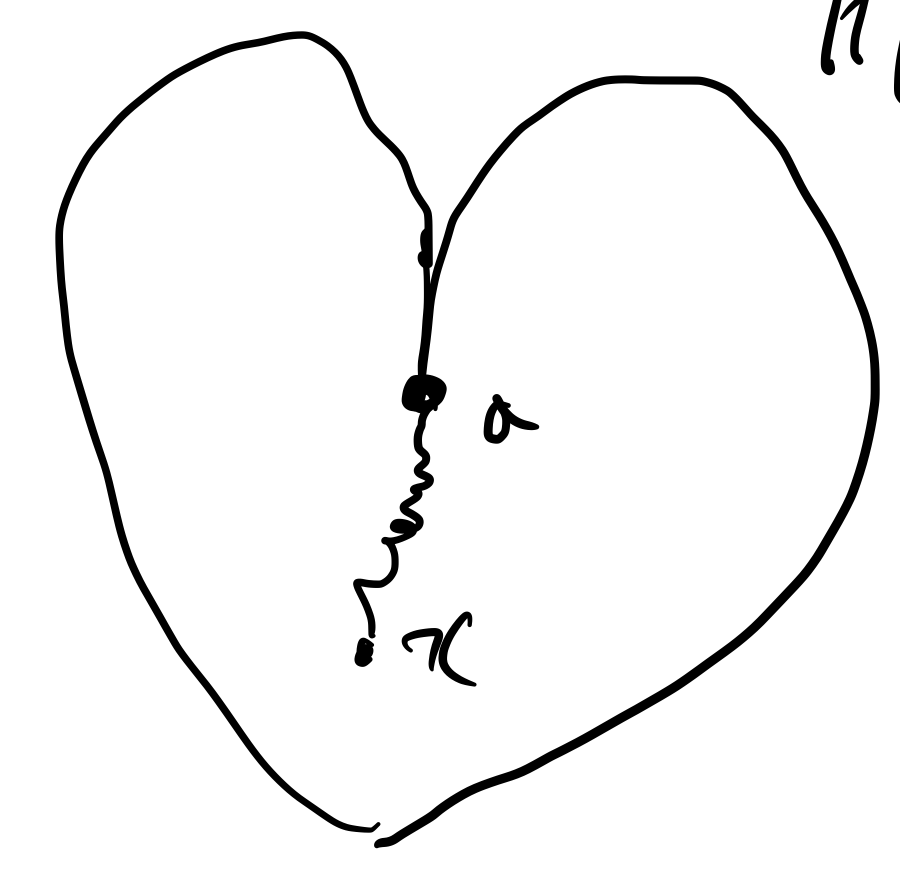
\includegraphics[width=0.25\textwidth]{heart.png}
    \caption{Heart shape domain}
    \label{fig:heart}
\end{figure}
\begin{dfn}{(Regular point)}
The point $a\in \partial D$ is \textbf{Regular} if 
\begin{equation*}
    \prob^a(\sigma_D) = 1,
\end{equation*} irregular if $\prob^a(\sigma_D) < 1$.
\end{dfn}

Also, by property of Brownian motion, and blumenthal 0-1 law, $\prob^a(\sigma_D)$ can only be 0 or 1.

\begin{example}
For one dimension, every point on $\partial D$ is regular. This can be proved by explicitly solving the PDE.
\end{example}

One way of checking this condition is Zaremba Cone condition:
We say that $a\in \partial D$ satisfies the condition if there exists $c(y, \theta) \in D^c$.
\begin{figure}[ht]
    \centering
    \includegraphics[width=0.4\textwidth]{cone.png}
    \caption{Cone}
\end{figure}
\begin{thm}
If a boundary point satisfies Zaremba Cone condition, then it is regular.
\end{thm}

\begin{thm}{(Continuity theorem)}
Let $d\geq 2, a\in\partial D$ then TFAE
\begin{itemize}
    \item For any $f: \partial D \rightarrow \R$ be bounded measurable and continuous at $a$ we have 
    \begin{equation*}
        \biglim{x\rightarrow a\in \partial D} \E^x f(W_{\tau_D}) = f(a).
    \end{equation*}
    \item $a$ is a regular point on $\partial D$.
\end{itemize}
\end{thm}
Then for an typical example of Dirichlet problem for Laplacian equation, we first have solution $u(x) = \E^x f(W_{\tau_D})$ then if every point on boundary is regular, we have that $u$ is continuous on closure of $D$ s.t. \begin{equation*}
    u\in C(\bar{D}).
\end{equation*}

\subsubsection{Poisson equation}
Now we switch from Brownian motion only to general SDE. Again, $D$ is open and bounded, now 
\begin{equation*}
\begin{cases}
    \diff X_t = F(X_t) \diff t + G(X_t) \diff W_t, \\
    X_0 = x \in D.
\end{cases}
\end{equation*}

Define generator for $\varphi \in C_b^2(D)$
\begin{equation*}
    L\varphi(x) = \frac{1}{2} Tr[G(x)G^*(x) \varphi_{xx}(x)] + \qvar{F(x), \varphi_x}{}.
\end{equation*}
The leaving time is still 
\begin{equation*}
    \tau_D := \inf\{t\geq 0; X_t^x \in \partial D \}.
\end{equation*}

\begin{dfn}{\textbf{Poisson equation in $D$ for $\lambda \geq 0$}}
\begin{equation*}
    \begin{cases}
        L u(x) - \lambda u(x) = -f(x) \quad & x\in D, \\
        u(x) = 0 \quad & x\in \partial D.
    \end{cases}
\end{equation*}
\end{dfn}

Then we have 
\begin{thm}
Assume $f\in C^2(\bar{D})$ and assume there exists a $C^2(\bar{D})$ solution $u$ to the Poisson equation then
\begin{equation*}
    u(x) = E^x \int_0^{\tau_D} e^{-\lambda s} f(X_s) \diff s, \quad \forall \lambda \geq 0,
\end{equation*} 
\end{thm}
with condition $\abs{G(x) h}^2 \geq c\abs{h}^2$ satisfied.

\begin{lem}
Assume there exists $c >0 \quad \abs{G(x) h}^2 \geq c\abs{h}^2, \forall x,h$ then the inverse exists and 
\begin{equation*}
    \norm{G^{-1}(x)} \leq \frac{1}{c}, \quad \forall x.
\end{equation*}
\end{lem}

In order to prove that $\boxed{\prob(\tau_D < \infty) = 1}$. That is, the process will leave the area $D$ a.s.

This is done by showing, in one specific direction, it will goes to infinity a.s. and this will be sufficient condition.

\subsection{Invariant measure}
For a random process $X_t$, if $\mu$ is invariant measure s,t, $x_0 \sim \mu$ then $X_t \sim \mu$.
\begin{equation*}
\begin{cases}
    \diff X_t = F(X_t) \diff t + G(X_t) \diff W_t, \\
    X_0 = x \in \R^d, t\geq 0.
\end{cases}
\end{equation*} $F, G$ Lipschitz.

\begin{dfn}{(Analytic definition of invariant measure)}
Invariant of probability distribution, for a process $X_t$
\begin{equation*}
    \int_{\R^d} P_t \varphi(x) \mu(\diff x) = \int_{\R^d} \varphi(x) \mu(\diff x).
\end{equation*}
\end{dfn}

\begin{thm} $(P_t)$ is a Feller semigroup iff $X(\cdot, x)$ is a Feller process, that is
\begin{equation*}
    \forall \varphi \in C_b(\R^d) \Leftrightarrow P_t\varphi \in C_b(\R^d).
\end{equation*}
\end{thm}
\pf See proof details \footnote{W11 L1}, then this can also be extended to bounded Borel function.
\begin{cor}
Let $\varphi$ be a bounded Borel function $(\varphi \in \B(\R^d))$ then $P_t\varphi \in \B(\R^d)$.
\end{cor}

\begin{dfn}{(Transition probability)}
\begin{equation*}
    \Pi_t(x, A) := \prob(X(t,x) \in A),
\end{equation*} then, we may write $X(t,x) \sim \Pi_t(x, \cdot)$.
\end{dfn}

Now i present an important derivation given $X_0 \sim \mu$ and $X_0$ independent of BM.
\begin{align*}
    \int_{\R^d} \varphi(x) \mu(\diff x) =& \E\varphi(X_t) = \E[\E(\varphi(X_t)| X_0)] \\
    =& \int_{\R^d} \E[\varphi(X(t,x))] \mu(\diff x) = \int_{\R^d} P_t \varphi(x) \mu(\diff x) \\
    =& \int_{\R^d} [\int_{\R^d} \varphi(y) \Pi_t(x, \diff y)] \mu(\diff x) = \int_{\R^d} \varphi(y) \int_{\R^d} \Pi_t(x, \diff y) \mu(\diff x),
\end{align*}
then, we may define $P_t^*\mu(A) := \int_{\R^d} \Pi_t(x, A) \mu(\diff x) $. Hence one can observe that 
\begin{itemize}
    \item $\varphi \rightarrow P_t\varphi$, how expected value evolves.
    \item $P_t^* \mu$ shows how distribution of $X$ evolves.
\end{itemize}

That is, if $\mu = P_t^* \mu, \forall t$ then $\mu$ is invariant. This gives another prospective of invariant measure.

\subsubsection{Existence of invariant measure}
There is no single answer to Existence or Uniqueness of invariant measure but we could still have following discussion.

\begin{assmp}\label{assmp: decreasing_map}
assume that 
\begin{equation*}
    2 \qvar{F(x) - F(y), x-y}{} + \abs{G(x) - G(y)}^2 \leq -\alpha \abs{x-y}^2, \alpha >0, \forall x,y.
\end{equation*}
\end{assmp}
Idea: The $F$ is a decreasing map and the diffusion part is relatively small that does not change the nature of decreasing map.

\begin{thm}
let the Assumption \ref{assmp: decreasing_map} be satisfied. Then there exists a unique invariant distribution for the process $X_t$. 
\end{thm}
The proof is interesting. At the end of the day, we can find
\begin{equation*}
    \E \abs{X_t^\lambda - \eta}^2 \xrightarrow{\lambda \rightarrow \infty} 0, \forall t.
\end{equation*}
Then we could say the $\mu$ is the invariant distribution, we could send $\lambda \rightarrow \infty$ then at any time $t$, $X \sim \mu$ which is exactly invariant measure. \footnote{W11 L1}

\begin{thm}{(Rate of convergence)}

let the Assumption \ref{assmp: decreasing_map} be satisfied and assume that $\varphi$ is Lipschitz,
\begin{equation*}
    \abs{\varphi(x) - \varphi(y)} \leq L\abs{x-y} 
\end{equation*}then for the invariant measure $\mu$ we have approximation
\begin{equation*}
    \abs{P_t \varphi(x) - \int_{\R^d} \varphi(y) \mu(\diff y)} \leq C(1+\abs{x} e^{-\alpha t} L).
\end{equation*}
\end{thm}
This is nice, now we could approximate the expectation value of process by using invariant measure as $t$ getting large. This property is handy since LHS is hard to measure but RHS is easy to do in real life.

\begin{thm}{(Prokhorov)}\label{thm: prokhorov}

Let $\{\mu_n; n\geq 1\}$ be a family of \textbf{probability measure} on $\R^d$. Then TFAE
\begin{itemize}
    \item There exists a sub-sequence $\mu_{n_{j}} \xrightarrow{w} \mu$ for a certain $\mu$.
    \item (Tightness condition) $\forall \epsilon >0$ these exists a \textbf{compact} set $K_\epsilon \subset \R^d$ s.t. 
    \begin{equation*}
        \mu_n(K_\epsilon) \geq 1-\epsilon, \forall n \geq 1.
    \end{equation*}
\end{itemize}
\end{thm}

\begin{cor}
It will be enough to show that $\forall \epsilon >0, \exists R_\epsilon$ s.t.
\begin{equation*}
    \prob(\abs{X_n} > R_\epsilon) < \epsilon, \forall n.
\end{equation*}
\end{cor}
\begin{cor}
It will be enough to show $M := \sup_n \E\abs{X_n} < \infty$ then apply Chebyshev inequality.
\end{cor}
\begin{thm}{(Krylov-Bogoliubov theorem)}
Assume that for a certain $x_0 \in \R^d$ the the family of measures 
$\{\Pi_t(x_0, \cdot); t\geq 0\}$ is tight then there exists an invariant (measure) distribution.
\begin{equation*}
    \int_{\R^d} P_t\varphi(x) \mu(\diff x) = \int_{\R^d} \varphi(x) \mu(\diff  x).
\end{equation*}
\end{thm}
\pf The proof is given by following schemes without details \footnote{detailed proof, see W11 L2}. Define averages of measures for $T >0$,
\begin{equation*}
    \mu_T(A) = \frac{1}{T}\int_0^T \Pi_t(x_0, A) \diff t.
\end{equation*}
\begin{enumerate}
    \item Show $\mu_T$ is a probability measure.
    \item The family $\{\mu_T ; T >0\}$ is tight.
\end{enumerate}
Then we have weak convergence subsequences by Thm \ref{thm: prokhorov} (Prokhorov), we claim this converging distribution is invariant measure. \qed

Comment: 
\begin{enumerate}
    \item The value have to be well-defined for all $x\in\R^d$, if it is not the case, then one have to check tightness condition or apply some transformations.
    \item No uniqueness can be guaranteed.
    \item Check for one specific starting point will be enough.
    \item Following conditions will all works $(c) \implies (a) \implies (b)$, $(c)$ is the most handy tool (easy to prove):
    \begin{enumerate}
        \item $\{\Pi_t(x_0, \cdot), t\geq 0\}$ is tight.
        \item $\{\mu_T(x_0, \cdot), T\geq 0\}$ is tight.
        \item $\boxed{M = \sup_{t \geq 0} \E\abs{X(t,x)} < \infty.}$
    \end{enumerate}
\end{enumerate}

Now we provide another way of showing existence of invariant measure.
\begin{dfn}\label{Lyapunov} Function $V: \R^d \rightarrow \R$ is Lyapunov function if
\begin{itemize}
    \item $V \in C^2(\R^d)$.
    \item $\biglim{\abs{x}\rightarrow \infty} V(x) = \infty$.
    \item By continuity and second property, WLOG $V(x) \geq 1$.
    \item $\exists a>0, c>0$ and $L$ is the generator of the process s.t.
    \begin{equation*}
        L V(x) \leq a - c V(x).
    \end{equation*}
\end{itemize}
\end{dfn} $L$-generator of the process with drift $F(x)$ and diffusion $G(x)$,
\begin{equation*}
    L\varphi(x) = \qvar{F(x), \varphi_x(x)}{} + \frac{1}{2} Tr[G(x) G^*(x) \varphi_{xx}(x)].
\end{equation*}
\begin{thm}{(Existence of invariant measure)}
Assume $X_t$ solves SDE uniquely and is Feller. Assume that there exists a Lyapunov function $V$ for this process. Then there exists an invariant measure.
\end{thm}
Note: Lipschitz continuous condition makes the solution unique and Feller.

\textbf{Comment: } Now we have two ways of testing existence of invariant measure, expected value of all $X_t$ or finding a Lyapunov function. Both way will be hard in general.

\subsubsection{Ergodicity and Von Neumann}

\begin{thm}{(Birkhoff Ergodic Theorem)}\label{Thm: BET}
Let $\mu$ be an invariant measure. Then for every $\varphi\in \ls{2}(\R^d, \mu)$ we have
\begin{equation*}
    \frac{1}{T} \int_0^T \varphi(X(t,x)) \diff t \xrightarrow{T\rightarrow \infty} \int_{\R^d} \varphi(x) \mu(\diff x) \quad \mu \text{ a.s. } x.
\end{equation*}
\end{thm}
Sometimes we write $\bar{\varphi} = \int_{\R^d} \varphi(x) \mu(\diff x)$.

\begin{dfn}{(Ergodicity and Strongly Mixing)}
We say that $\mu$ is ergodic if $\forall \varphi \in \ls{2}(\R^d,\mu)$
\begin{equation*}
    \biglim{T\rightarrow \infty} \frac{1}{T} \int_0^T P_t \varphi \diff t = \int_{\R^d} \varphi(x) \mu(\diff x).
\end{equation*}
$\mu$ is strongly mixing if 
\begin{equation*}
    \biglim{T\rightarrow \infty} P_t \varphi \diff t = \int_{\R^d} \varphi(x) \mu(\diff x).
\end{equation*}
\end{dfn}
We denote the norm of random variable as
\begin{equation*}
    \norm{\varphi}_2 = (\int_{\R^d} \varphi^2(x) \diff x)^{\frac{1}{2}}.
\end{equation*}

\begin{thm}
More than  Feller, we also have $\varphi \in \ls{2}(\R^d,\mu) \implies P_t\varphi \in \ls{2}(\R^d,\mu) $ and the semigroup operator $P_t$ is a \textbf{contraction} s.t.
\begin{equation*}
    \norm{P_t\varphi}_2 \leq \norm{\varphi}_2.
\end{equation*}
\end{thm}

\begin{dfn}
We say a process $f$ is $P_t-$ harmonic or $L-$ harmonic process if a process $f\in \Sigma$ s.t.
\begin{equation*}
    \Sigma := \{f\in \ls{2}(\R^d, \mu); P_t f = f, \mu-a.s.\}.
\end{equation*}
\end{dfn}
$L$-generator of the process.
\begin{equation*}
    L\varphi(x) = \qvar{F(x), \varphi_x(x)}{} + \frac{1}{2} Tr[G(x) G^*(x) \varphi_{xx}(x)].
\end{equation*}
Properties of $\Sigma$:
\begin{itemize}
    \item $f\in \Sigma \implies L f = 0$.
    \item Constants are in $\Sigma$.
    \item $\Sigma$ is closed in $\ls{2}(\R^d,\mu)$. That is $f_n \in \Sigma$ and $f_n \xrightarrow{\ls{2}} f$ then $f\in \Sigma$.
\end{itemize}
\pf Recall $\frac{\diff}{\diff t} P_t \varphi = L P_t \varphi$, then 
\begin{equation*}
    \biglim{t\rightarrow 0} \frac{P_t \varphi - \varphi}{t} = L\varphi.
\end{equation*}Therefore $L \varphi = 0$. 
\qed

More properties, Let $\varphi, \psi \in \Sigma$:
\begin{itemize}
    \item Closed under addition and multiplication of integers.
    \item $\abs{\varphi} \in \Sigma$.
    \item $\varphi^+, \varphi^- \in \Sigma$.
    \item $\varphi \wedge \psi, \varphi \vee \psi\in \Sigma$.
    \item $\forall a\in \R, \I{\{\varphi > a\}} \in \Sigma$.
\end{itemize}
\pf 
\begin{align*}
    &\varphi^+ = \frac{1}{2}(\varphi + \abs{\varphi}) &\varphi^- = \frac{1}{2}(\varphi - \abs{\varphi}) \\
    &\varphi \wedge \psi = (\varphi - \psi)^+ + \varphi &\varphi \vee \psi = (\varphi - \psi)^+ + \psi
\end{align*}
\begin{thm}{(Von Neumann)}
Let $\mu$ be invariant measure, $\forall \varphi \in \ls{2}(\R^d,\mu)$ there exists the limit
\begin{equation*}
    \biglim{T\rightarrow \infty} M(T)\varphi \xrightarrow{\ls{2}} M_\infty \varphi,
\end{equation*} equivalently
\begin{equation*}
    \biglim{T\rightarrow \infty} \frac{1}{T} \int_0^T P_t \varphi \diff t \xrightarrow{\ls{2}} M_\infty \varphi,
\end{equation*}
with $M(T)\varphi = \frac{1}{T} \int_0^T P_t \varphi \diff t$. Moreover, $M_\infty$ is projections on space $\Sigma$.
\begin{itemize}
    \item $M_\infty^2 \varphi = M_\infty \varphi$.
    \item $M_\infty \varphi \in \Sigma$.
    \item $\int_{\R^d} M_\infty \varphi(x) \mu(\diff x) =  \int_{\R^d} \varphi(x) \mu(\diff x)$.
\end{itemize}
$\mu$ is ergodic if $M_\infty\varphi = \int \varphi(x) \mu(\diff x)$, here 
\begin{equation*}
    \int_{\R^d} M_\infty \varphi(x) \mu(\diff x) = M_\infty\varphi \implies M_\infty \varphi \text{ constant}.
\end{equation*}
\end{thm}

\begin{prop}
Let $\mu$ be invariant measure then $\mu$ is \textbf{ergodic} iff $\Sigma$ is \textbf{one dimensional} then it is ergodic:
\begin{equation*}
    \Sigma = \{ cf; c\in \R \}.
\end{equation*}
\end{prop}

\pf It contains functional analysis thus omitted. Since the $\Sigma$ is one dimensional, it only contains constant, thus $M_\infty\varphi \in \Sigma$ and $\int_{\R^d} M_\infty \varphi(x) \mu(\diff x) = M_\infty\varphi(x) =  \int_{\R^d} \varphi(x) \mu(\diff x)$, it is then clear.
\qed

\begin{dfn}
A Borel set $B\subset \R^d$ is \textbf{invariant} for $(P_t)$ if $\I{B} \in \Sigma$. We say $B$ is \textbf{trivial} if
\begin{equation*}
    \mu(B) = 0 \quad \text{ or } \quad \mu(B) = 1.
\end{equation*}
\end{dfn}
Connect the idea from Markov chain since 
\begin{equation*}
    \I{B} \in \Sigma \implies P_t \I{B}(x) = \I{B}(x) \implies \prob(X(t,x) \in B) =  \I{B}(x).
\end{equation*}
That is, if $X$ starts in $B$ it stays here forever, if it starts somewhere else, it will never enter $B$. Hence, $B$ is non trivial iff there is no proper subsets of $\R^d$ invariant for the evolution of the process. (Cannot reduced the space.)

\begin{thm} Let $\mu$ be invariant measure then $\mu$ is \textbf{ergodic} iff all invariant sets are \textbf{Trivial}.
\end{thm}

\begin{thm} Let $\mu$ be \textbf{unique} then it is ergodic s.t.
\begin{equation*}
    \frac{1}{T} \int_0^T P_t\varphi \diff t \xrightarrow{T\rightarrow \infty} \bar{\varphi}.
\end{equation*}
\end{thm}
\pf Idea: if $\mu$ not ergodic, then some invariant sets are non trivial, we could construct a conditional measure on this set that are different from $\mu$. This lead to a contradiction to the uniqueness.

\newpage
\subsubsection{Uniqueness of invariant measure}
\textbf{Question: } When the invariant measure $\mu$ is unique? 

\textbf{Answer: }If $X$ is irreducible and strongly Feller. This subsection will introduce this two main results.
\begin{dfn}
The solution to an SDE is \textbf{irreducible} if for every $x\in\R^d, \forall t>0, \forall y \in \R^d, \forall r >0$,
\begin{equation*}
    \prob(\abs{X(t,x) - y} <r) >0.
\end{equation*}.
\end{dfn}

Similar to Markov Chain, if the process can get to any point in the space arbitrarily close. Then it is irreducible (cannot reduce the space). In other words, the density (if exists) does not vanishes anywhere.

\begin{example}
One/two dimensional Brownian motion, three dimensional Brownian motion is not irreducible. 
\end{example}

One possible way of proving this is by utilizing Girsanov theorem. See W12 L2 page 5 for details. We could use this idea to form a theorem.

\begin{thm}
Assume that SDE with following structure
\begin{equation*}
    \begin{cases}
        \diff X_t = F(X_t) \diff t + G \diff W_t, \\
        X_0 = x \in \R^d.
    \end{cases}
\end{equation*}
Let $G^{-1}$ exist and $\abs{F(x)} \leq c(1+\abs{x})$ then $X$ is irreducible.
\end{thm}

Note here $G$ is constant matrix/ value and $F$ satisfies linear growth rate.
\begin{thm}
Assume that SDE with following structure:
\begin{equation*}
    \begin{cases}
        \diff X_t = F(X_t) \diff t + G(X_t) \diff W_t, \\
        X_0 = x \in \R^d.
    \end{cases}
\end{equation*}
Assume that 
\begin{equation*}
    \sup_{x} \abs{G^{-1}(x)F(x)} <\infty,
\end{equation*}
then $X$ is irreducible.
\end{thm}

\begin{dfn}{(Strong Feller)}\label{dfn: strongfeller}

A process of semigroup $P_t$ is called strong Feller if  
\begin{equation*}
    \varphi \text{ bounded Borel} \implies P_t \varphi \in C_b(\R^d).
\end{equation*}
\end{dfn}
Comment: the transition semigroup "improved" the process.

\begin{thm}
Let $X(\cdot, x)$ be solution to any SDE and assume that $X(t,x)$ has a density $p_t(x,y)$ \textbf{continuous} and \textbf{bounded} then it is strong Feller.
\end{thm}

\pf The proof is straightforward,
\begin{equation*}
    P_t\varphi(x) = \E\varphi(X(t,x)) = \int_{\R^d} \varphi(y) p_t(x,y) \diff y.
\end{equation*}
Since the density and $\varphi$ are bounded, we use Fubini theorem to obtain continuity of $P_t\varphi$ 
\qed

\begin{example}{(Ornstein–Uhlenbeck process)}

Refers to the example at \ref{example: OUprocess}, 
\begin{equation*}
    X_t = e^{tA}x + \int_0^t e^{(t-s)A}B \diff W_s,
\end{equation*}
and,
\begin{equation*}
    X_t \sim N(e^{tA}x, \int_0^t e^{sA} BB^* e^{sA^*} \diff s).
\end{equation*} denote the covariance matrix as $Q_t$
Then if $\det(Q_t)>0$, $X(t,x)$ has multi Gaussian density which makes $X_t$ Feller.
\end{example}


\begin{thm}
Assume $F\in C^1(\R^d, \R^d)$ and Lipschitz, let $F_x$ be bounded, $G\in C_b^1(\R^d, \R^d \otimes \R^d)$, $\exists c >0$ s.t. $\abs{G(x) h} \geq c\abs{h}^2, \forall h,x\in R^d$ and $\abs{G^{-1}(x)} \leq \frac{1}{\sqrt{c}}$, then $(P_t)$ is strong Feller.
\end{thm}
\vspace{1cm}
Now we move to the main result of uniqueness of invariant measure.
\begin{thm}
Assume $P_t$ is strong Feller and irreducible. Then $\Pi(x, \cdot), \Pi(y, \cdot)$ are equivalent $\forall t>0, \forall x,y\in\R^d$.
\end{thm}
\pf See W13 L1, if I have time I will come back to fill this, ow see the lecture notes. This is a very good proof using strong Feller and irreducibility.

\begin{thm}{(Uniqueness)}
Let $P_t$ be strong Feller and irreducible. Let $\mu$ be an invariant measure. Then 
\begin{itemize}
    \item $\mu$ is equivalent to any measure $\Pi_t(x,\cdot), \forall t>0, \forall x\in\R^d.$
    \item $\mu$ is the \textbf{unique} ergodic invariant measure.
\end{itemize}
\end{thm}
Logic: If $P_t$ is strong Feller and irreducible, then if invariant measure $\mu$ exist, it is unique and thus ergodic and strongly mixing and 
\begin{equation*}
    \forall x \in \R^d, \forall B\in\B(\R^d), \prob(X(t,x)\in B) \xrightarrow{t\rightarrow\infty} \mu(B).
\end{equation*}

\begin{lem}
Assume $\mu_1, \mu_2$ are two ergodic invariant measures, then $\mu_1 \perp \mu_2$. 
\end{lem}
The symbol $\perp$ stands for singular relationship (in contrast to equivalence), s.t. there exists two sets $A, B, \mu_1(A) = \mu_2(B) = 1, A\cap B = \emptyset$.

\begin{thm}{(Uniqueness)}\label{Thm: uniqueness}
Let $\mu$ be an invariant measure and let $P_t$ be strongly Feller and irreducible, then the invariant measure is \textbf{unique} hence \textbf{ergodic}, moreover $\mu$ is \textbf{strongly mixing} and
\begin{equation*}
    \prob(X(t,x)\in B) \xrightarrow{t\to \infty} \mu(B),\quad \forall x\in\R^d, \forall B\subset \R^d.
\end{equation*}
\end{thm}

\subsubsection{Properties of invariant measure}
Lastly, we study the property of set of invariant measure. 
\begin{itemize}
    \item The set of invariant measure is convex, if $\mu_1, \mu_2$ invariant, then $\mu := p_1\mu_1 + p_2 \mu_2$ is also invariant.
    \item The set of invariant measure is closed.
\end{itemize}

\begin{thm}{(Extremal point)}
Let $E$ be Banach space and let $C \subset E$ be convex, the point $x$ is \textbf{external} if $x$ can not be written in the form of 
\begin{equation*}
    x = p y_1 +(1-p) y_2, p\in(0,1), y_1, y_2 \in C.
\end{equation*}
\end{thm}

\begin{thm}{(Krein–Milman theorem)}

Let $C$ be a closed, convex set in a Banach space $E$ then every point $x\in C$ is a convex combination of \textbf{extremal} points:
\begin{equation*}
    x = \bigs{k=1}^n p_k e_k, p_k \geq 0, \sum_{k} p_k =1, e_k \text{ extremal points}.
\end{equation*}
\end{thm}

\begin{thm}
Let $C$ be the set of invariant measure, then $\mu \in C$ is ergodic iff $\mu$ is an extremal point.
\end{thm}
An immediate consequence is that every other invariant measures in convex combinations of ergodic invariant measures.

\subsubsection{Density of invariant measures}
This part will rather be brief introduction of Fokker–Planck equation. This equation gives an representation of general formula of density of invariant measures in PDE, see W13 L1 for details.